% ══════════════════════════════════════════════════════════════════════════════
%  CS495-Capstone-Poster.tex
%  CS495 -- Data Science Project Practicum
%  Capstone Poster -- Bellevue College
%  Size:  36" x 48" portrait
%  Build: pdflatex CS495-Capstone-Poster.tex      (run twice)
%
%  Based on CS495-Poster-Template.tex (BC brand chrome).
%  Embedded figures retain the project's navy / skyblue palette.
% ══════════════════════════════════════════════════════════════════════════════

\documentclass[a0,portrait]{a0poster}

% ── Override paper to 36" x 48" portrait ──────────────────────────────────────
\setlength{\paperwidth}{36in}
\setlength{\paperheight}{48in}
\special{papersize=36in,48in}

% ---------- Packages ----------
\usepackage[utf8]{inputenc}
\usepackage[T1]{fontenc}
\usepackage[english]{babel}
\usepackage{graphicx}
\usepackage{amsmath,amssymb}
\usepackage{booktabs}
\usepackage{array}
\usepackage{multicol}
\usepackage{xcolor}
\usepackage{enumitem}
\usepackage{tcolorbox}
\usepackage{tikz}
\usetikzlibrary{positioning, arrows.meta, calc}
\usepackage{ragged2e}
\usepackage{anyfontsize}
\usepackage{qrcode}
\tcbuselibrary{skins,breakable}

% ── Page geometry override for 36"x48" ────────────────────────────────────────
\setlength{\hoffset}{-1in}
\setlength{\voffset}{-1in}
\setlength{\oddsidemargin}{2cm}
\setlength{\evensidemargin}{2cm}
\setlength{\topmargin}{2cm}
\setlength{\headheight}{0pt}
\setlength{\headsep}{0pt}
\setlength{\topskip}{0pt}
\setlength{\textwidth}{\dimexpr\paperwidth-4cm\relax}
\setlength{\textheight}{\dimexpr\paperheight-4cm\relax}

% ---------- Bellevue College Brand Colors ----------
\definecolor{BCBlue}{HTML}{003D79}        % Brutus Blue   (primary)
\definecolor{BCSilver}{HTML}{A7A9AC}      % Bulldog Silver (primary)
\definecolor{BCRed}{HTML}{C4122F}         % Fall Maple Red (accent)
\definecolor{BCLightBlue}{HTML}{E6EEF7}   % Soft tinted background
\definecolor{BCDarkBlue}{HTML}{002851}    % Deeper variant
\definecolor{BCInk}{HTML}{1A1A1A}         % Body text

% ---------- Layout ----------
\setlength{\parindent}{0pt}
\setlength{\parskip}{0.3em}
\setlength{\columnsep}{2.0cm}
\setlength{\columnseprule}{0pt}

% ---------- Block container (BC brand chrome) ----------
\newtcolorbox{posterblock}[1]{
    enhanced, breakable,
    colback=white, colframe=BCSilver,
    boxrule=0.8pt, arc=6pt,
    left=14pt, right=14pt, top=6pt, bottom=10pt,
    fonttitle=\bfseries\Large,
    title={#1},
    coltitle=white,
    colbacktitle=BCBlue,
    attach boxed title to top left={xshift=0mm, yshift=0mm},
    boxed title style={
        colback=BCBlue, colframe=BCBlue,
        sharp corners, boxrule=0pt,
        left=14pt, right=18pt, top=6pt, bottom=6pt,
    },
    title filled=true,
    before skip=10pt, after skip=10pt,
    overlay unbroken and first={
        \fill[BCRed] (frame.north west) rectangle ([xshift=12pt]frame.north west|-title.south);
    },
}

% ---------- Inline tinted callout (for equations / key facts) ----------
\newtcolorbox{callout}{
    colback=BCLightBlue, colframe=BCLightBlue,
    arc=4pt, left=14pt, right=14pt, top=10pt, bottom=10pt,
    boxrule=0pt,
}

% ══════════════════════════════════════════════════════════════════════════════
\begin{document}

% ══════════════════════════════════════════════════════════════════════════════
%  TITLE BANNER
% ══════════════════════════════════════════════════════════════════════════════
\noindent

\begin{tikzpicture}[remember picture]
  \fill[BCLightBlue] (0,0) rectangle (\textwidth, 11cm);
  \fill[BCRed]  (0,0) rectangle (\textwidth, 0.6cm);

  % Bellevue College logo on the left
  \node[anchor=west, inner sep=0pt] at (1cm, 6cm) {
    \IfFileExists{BellevueCollegeLogoHorzClr.png}{%
      \includegraphics[height=7cm]{BellevueCollegeLogoHorzClr.png}%
    }{%
      \colorbox{BCDarkBlue}{\parbox[c][7cm][c]{22cm}{\centering\bfseries
        \color{BCBlue}\fontsize{50}{60}\selectfont Bellevue College}}%
    }
  };

  % Title text on the right --- FULL width (the headline stays prominent)
  \node[anchor=west, inner sep=0pt, text width=\textwidth-32cm, align=left]
       at (32cm, 8.2cm) {%
    \color{BCDarkBlue}\fontsize{60}{72}\selectfont\bfseries
    Mathematical and Empirical Models in Agreement
  };

  % Subtitle / author / course --- narrowed by ~7 cm to make room for the QR
  \node[anchor=west, inner sep=0pt, text width=\textwidth-39cm, align=left]
       at (32cm, 5.0cm) {%
    \color{BCDarkBlue}\fontsize{36}{44}\selectfont
    Cross-Validating CRR Binomial Pricing and Machine Learning\\
    for Crowd Mispricing Detection in Equity Options
  };
  \node[anchor=west, inner sep=0pt, text width=\textwidth-39cm, align=left]
       at (32cm, 2.7cm) {%
    \color{BCDarkBlue}\fontsize{30}{36}\selectfont
    \textbf{Author:} DeWayne Dantzler \quad\textbar\quad
    \textbf{Faculty Advisor:} Dr.~Pedro Albuquerque
  };
  \node[anchor=west, inner sep=0pt, text width=\textwidth-39cm, align=left]
       at (32cm, 1.2cm) {%
    \color{BCDarkBlue}\fontsize{24}{30}\selectfont\itshape
    CS\,495 -- Data Science Project Practicum \;\textbullet\;
    Bellevue College \;\textbullet\; Spring 2026
  };

  % QR code on the far right side of the banner, vertically centered on the subtitle block
  \node[anchor=east] at (\textwidth - 1cm, 4.5cm)
       {\fbox{\qrcode[height=5cm]{https://github.com/dantzlerdc/CS495-Deep-Scholar}}};
\end{tikzpicture}

\vspace{2cm}

% ══════════════════════════════════════════════════════════════════════════════
%  THREE-COLUMN BODY
% ══════════════════════════════════════════════════════════════════════════════
\RaggedRight
\normalsize
\enlargethispage{4cm}

\begin{multicols}{3}

% ──────────────────────────────────────────────────────────────────────────────
%  LEFT COLUMN
% ──────────────────────────────────────────────────────────────────────────────

\begin{posterblock}{Abstract}
This project addresses a foundational question in quantitative finance:
when an options pricing model produces a theoretical fair value that
diverges from the observed market premium, is that divergence large
enough --- and reliable enough --- to justify a trade? A Cox--Ross--%
Rubinstein (CRR) American binomial option pricer is built in vectorized
Python and validated against a live AMD option chain from Fidelity
(April 2026). Its mispricing-edge signal is then cross-validated against
an independent XGBoost ITM/OTM probability classifier trained on
101{,}535 historical AAPL contracts. The two layers agree strongly in
the herding regime (Pearson correlation $r=0.413$,
$p=2.4\times10^{-10}$) and not at all in the normal regime ($r\approx0$).
A regime-conditioned Kelly Criterion framework converts the
cross-validated edge into risk-controlled capital allocation.

\vspace{0.4em}
\textbf{Keywords:} CRR binomial pricing, options mispricing, XGBoost,
Kelly Criterion, behavioral finance, EMH, herding regime.
\end{posterblock}

\begin{posterblock}{Introduction \& Motivation}
Options markets aggregate beliefs into prices much like prediction
markets do, but behavioral forces --- herding around round strikes,
implied-volatility overpricing driven by fear, and systematic skew in
out-of-the-money puts --- distort prices in predictable ways. The gap
between a pricing model's theoretical fair value and the observed
market premium is potentially exploitable by a disciplined, model-driven
strategy, but only if the divergence is large enough, reliable enough,
and detectable by independent methods.

\vspace{0.5em}
\textbf{Research Questions}
\begin{itemize}[leftmargin=1.4em,itemsep=4pt,topsep=4pt]
  \item Do CRR model prices predict whether an equity option expires
        in-the-money or out-of-the-money?
  \item Does cross-validation between CRR (math) and an ML classifier
        detect exploitable pricing \emph{edge}?
  \item Does regime-conditioned Kelly sizing convert that edge into
        positive expected value?
\end{itemize}

\vspace{0.3em}
\textbf{Objectives}
\begin{itemize}[leftmargin=1.4em,itemsep=4pt,topsep=4pt]
  \item Implement the CRR American binomial lattice (no dividends) in
        vectorized Python at $N=100$ steps.
  \item Validate pricing accuracy against AMD market premiums within
        $\pm 5\%$ error.
  \item Train an XGBoost ITM/OTM classifier on engineered features
        \emph{without} using IV as an input (independence from L1).
  \item Apply Kelly Criterion (full / half / quarter) for
        risk-controlled position sizing.
\end{itemize}
\end{posterblock}

\begin{posterblock}{Monte Carlo Simulation}
A Monte Carlo simulation validates that the Kelly Criterion converts
the cross-validated edge into positive expected value under realistic
trade-by-trade dynamics. One thousand trades are drawn from the
empirical edge distribution with $p_{\text{win}} = 0.677$, and the
cumulative profit-and-loss is tracked under full-, half-, and
quarter-Kelly position sizing.

\vspace{0.3em}
\begin{center}
  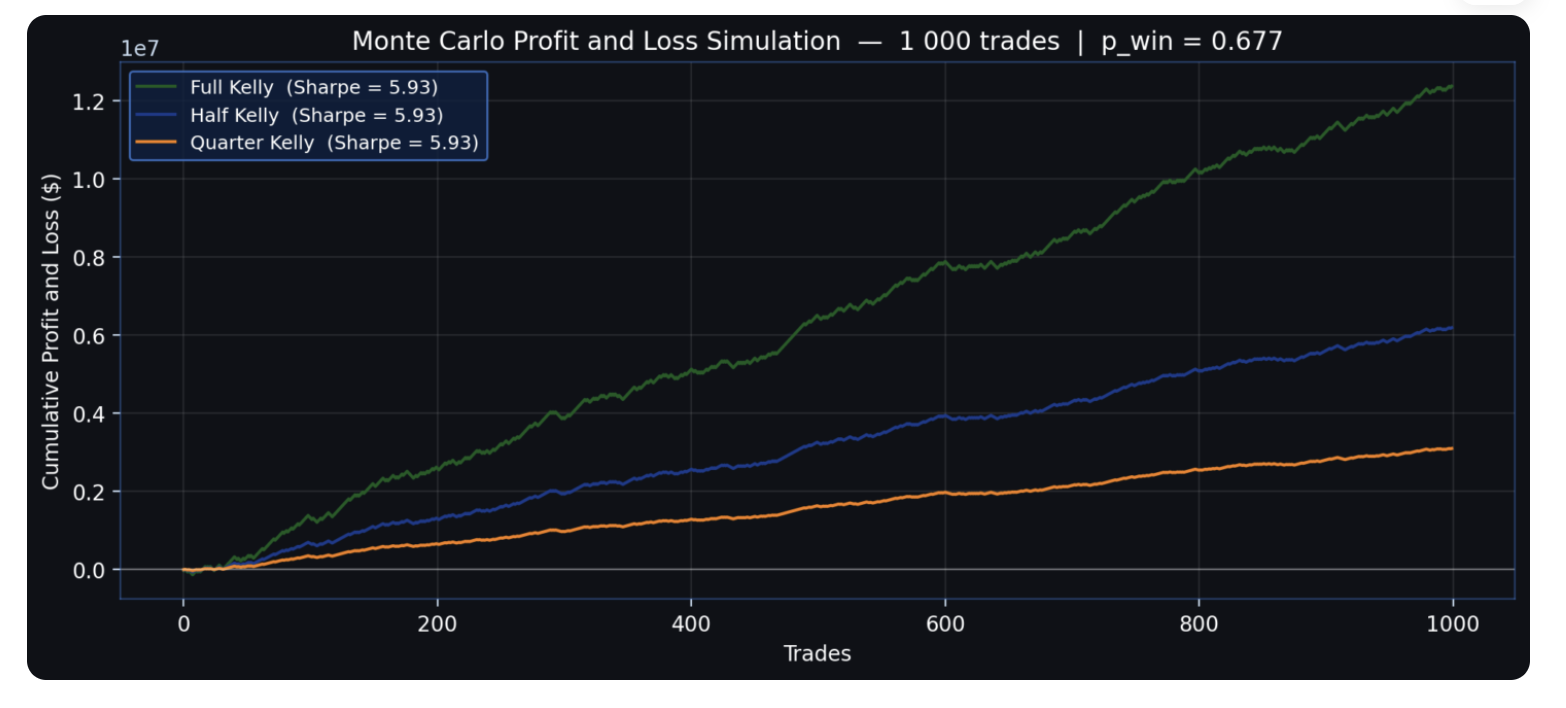
\includegraphics[width=0.78\linewidth,keepaspectratio]
    {PosterFigures/CRR-Monte-Carlo-Simulation.png}
\end{center}

\vspace{0.2em}
\textbf{Reading the curves.} Full Kelly (green) reaches $\sim\$12$M;
half-Kelly (blue) \$6M; quarter-Kelly (orange) \$3M. All three
variants share Sharpe $=5.93$, confirming the Kelly fraction trades
absolute return for drawdown control without changing risk-adjusted
performance. The live pipeline runs half-Kelly in normal regimes and
quarter-Kelly in herding regimes to keep the realized max drawdown
below the $15\%$ circuit-breaker threshold.
\end{posterblock}

\begin{posterblock}{Exploratory Data Analysis}
Cross-validating the two independent edge signals on $3{,}000$ AAPL
contracts reveals the central empirical finding of the project: the
two models agree on direction precisely in the \emph{herding} regime
(red), not in the \emph{normal} regime (blue).

\vspace{0.3em}
\begin{center}
  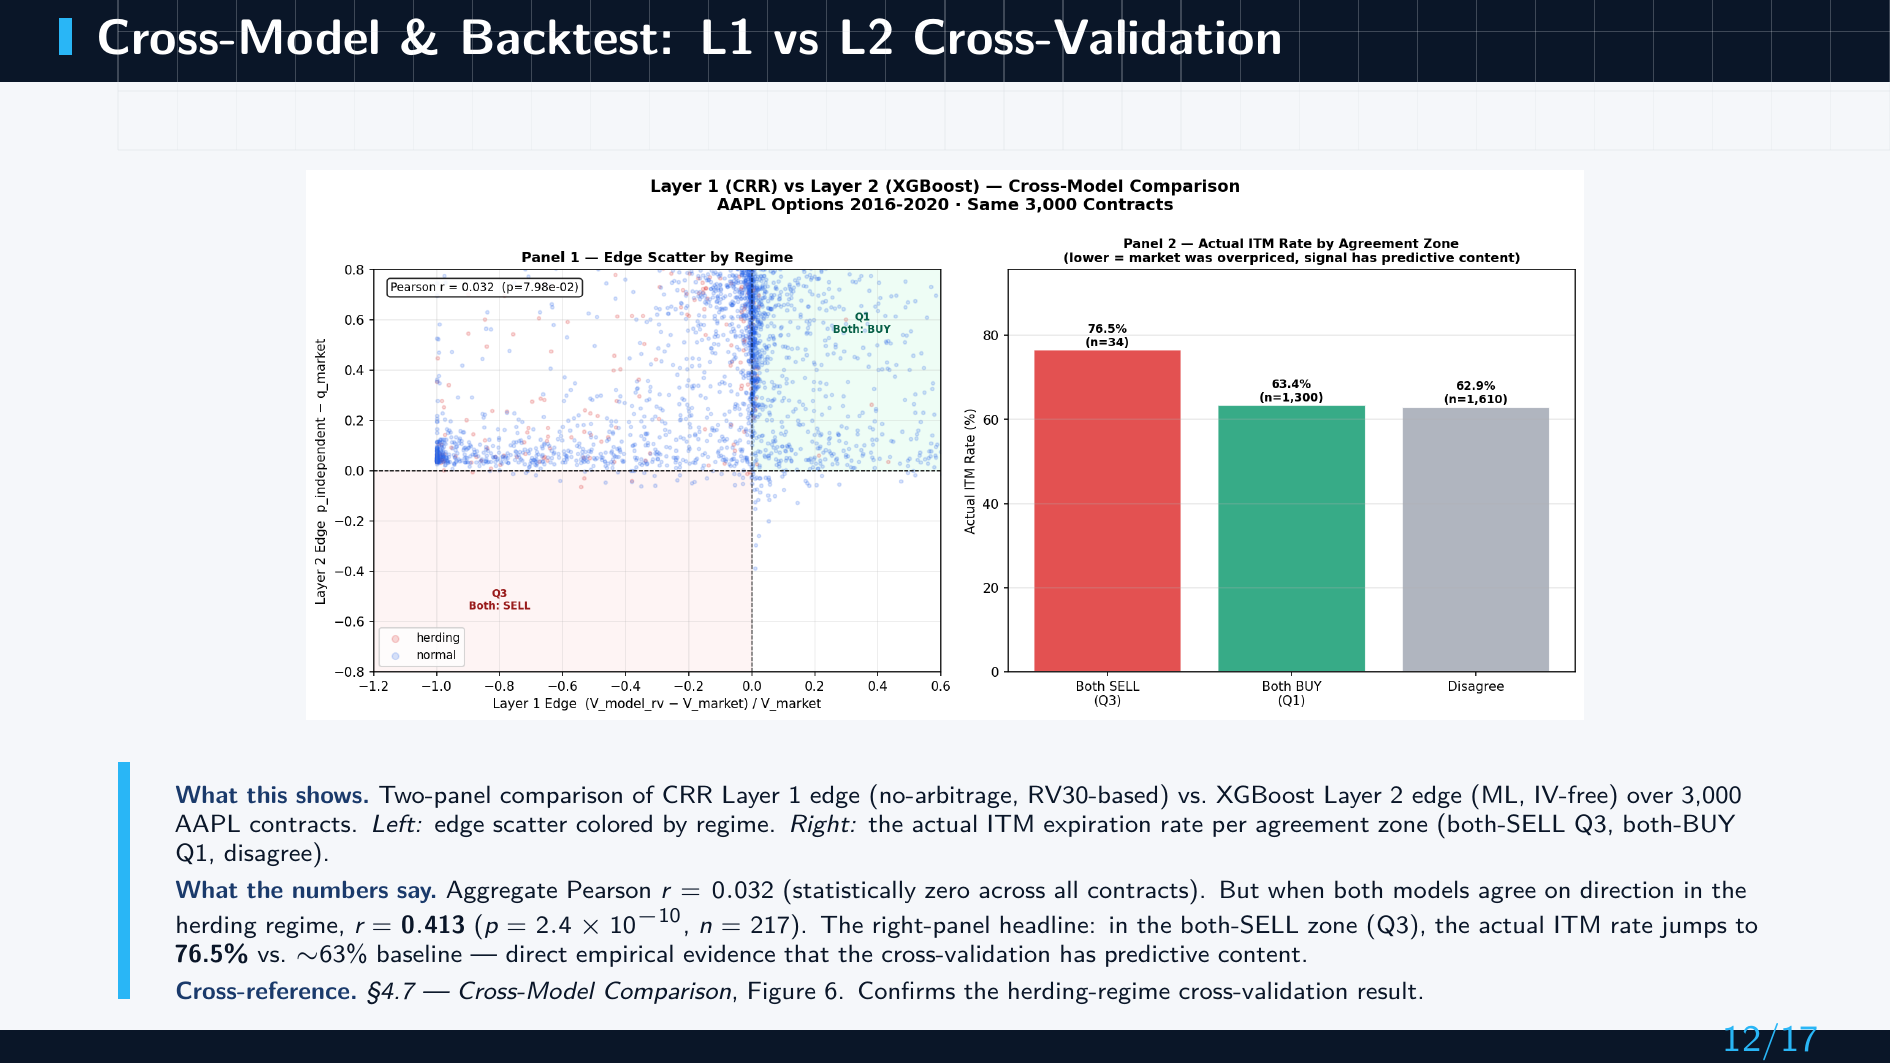
\includegraphics[width=0.78\linewidth,keepaspectratio]
    {PosterFigures/Slide12-L1vsL2.png}
\end{center}

\vspace{0.3em}
\textbf{Key pattern.} \emph{Left panel:} Layer-1 vs Layer-2 edge
scatter colored by regime; the pooled Pearson correlation is
$r=0.032$ ($p=0.080$), statistically zero across all contracts.
\emph{Right panel:} the actual ITM expiration rate per agreement
zone --- when both layers say SELL (Q3, $n=34$), the realized ITM
rate jumps to $\mathbf{76.5\%}$ versus the $\sim 63\%$ baseline. The
aggregate-vs-conditional inversion is a textbook Simpson's paradox:
$r$ rises to $\mathbf{0.413}$ ($p=2.4\times 10^{-10}$, $n=217$)
once herding-regime contracts are isolated. This is the empirical
fingerprint of \emph{Samuelson macro-inefficiency} --- markets are
micro-efficient on average but exhibit aggregate bias under
coordinated behavioral demand.
\end{posterblock}

% ──────────────────────────────────────────────────────────────────────────────
\columnbreak
%  CENTER COLUMN
% ──────────────────────────────────────────────────────────────────────────────

\begin{posterblock}{Methodology}
A three-layer pipeline runs CRR and XGBoost independently, then merges
their edge signals through a regime-conditioned Kelly position sizer.

\vspace{0.3em}
\begin{center}
  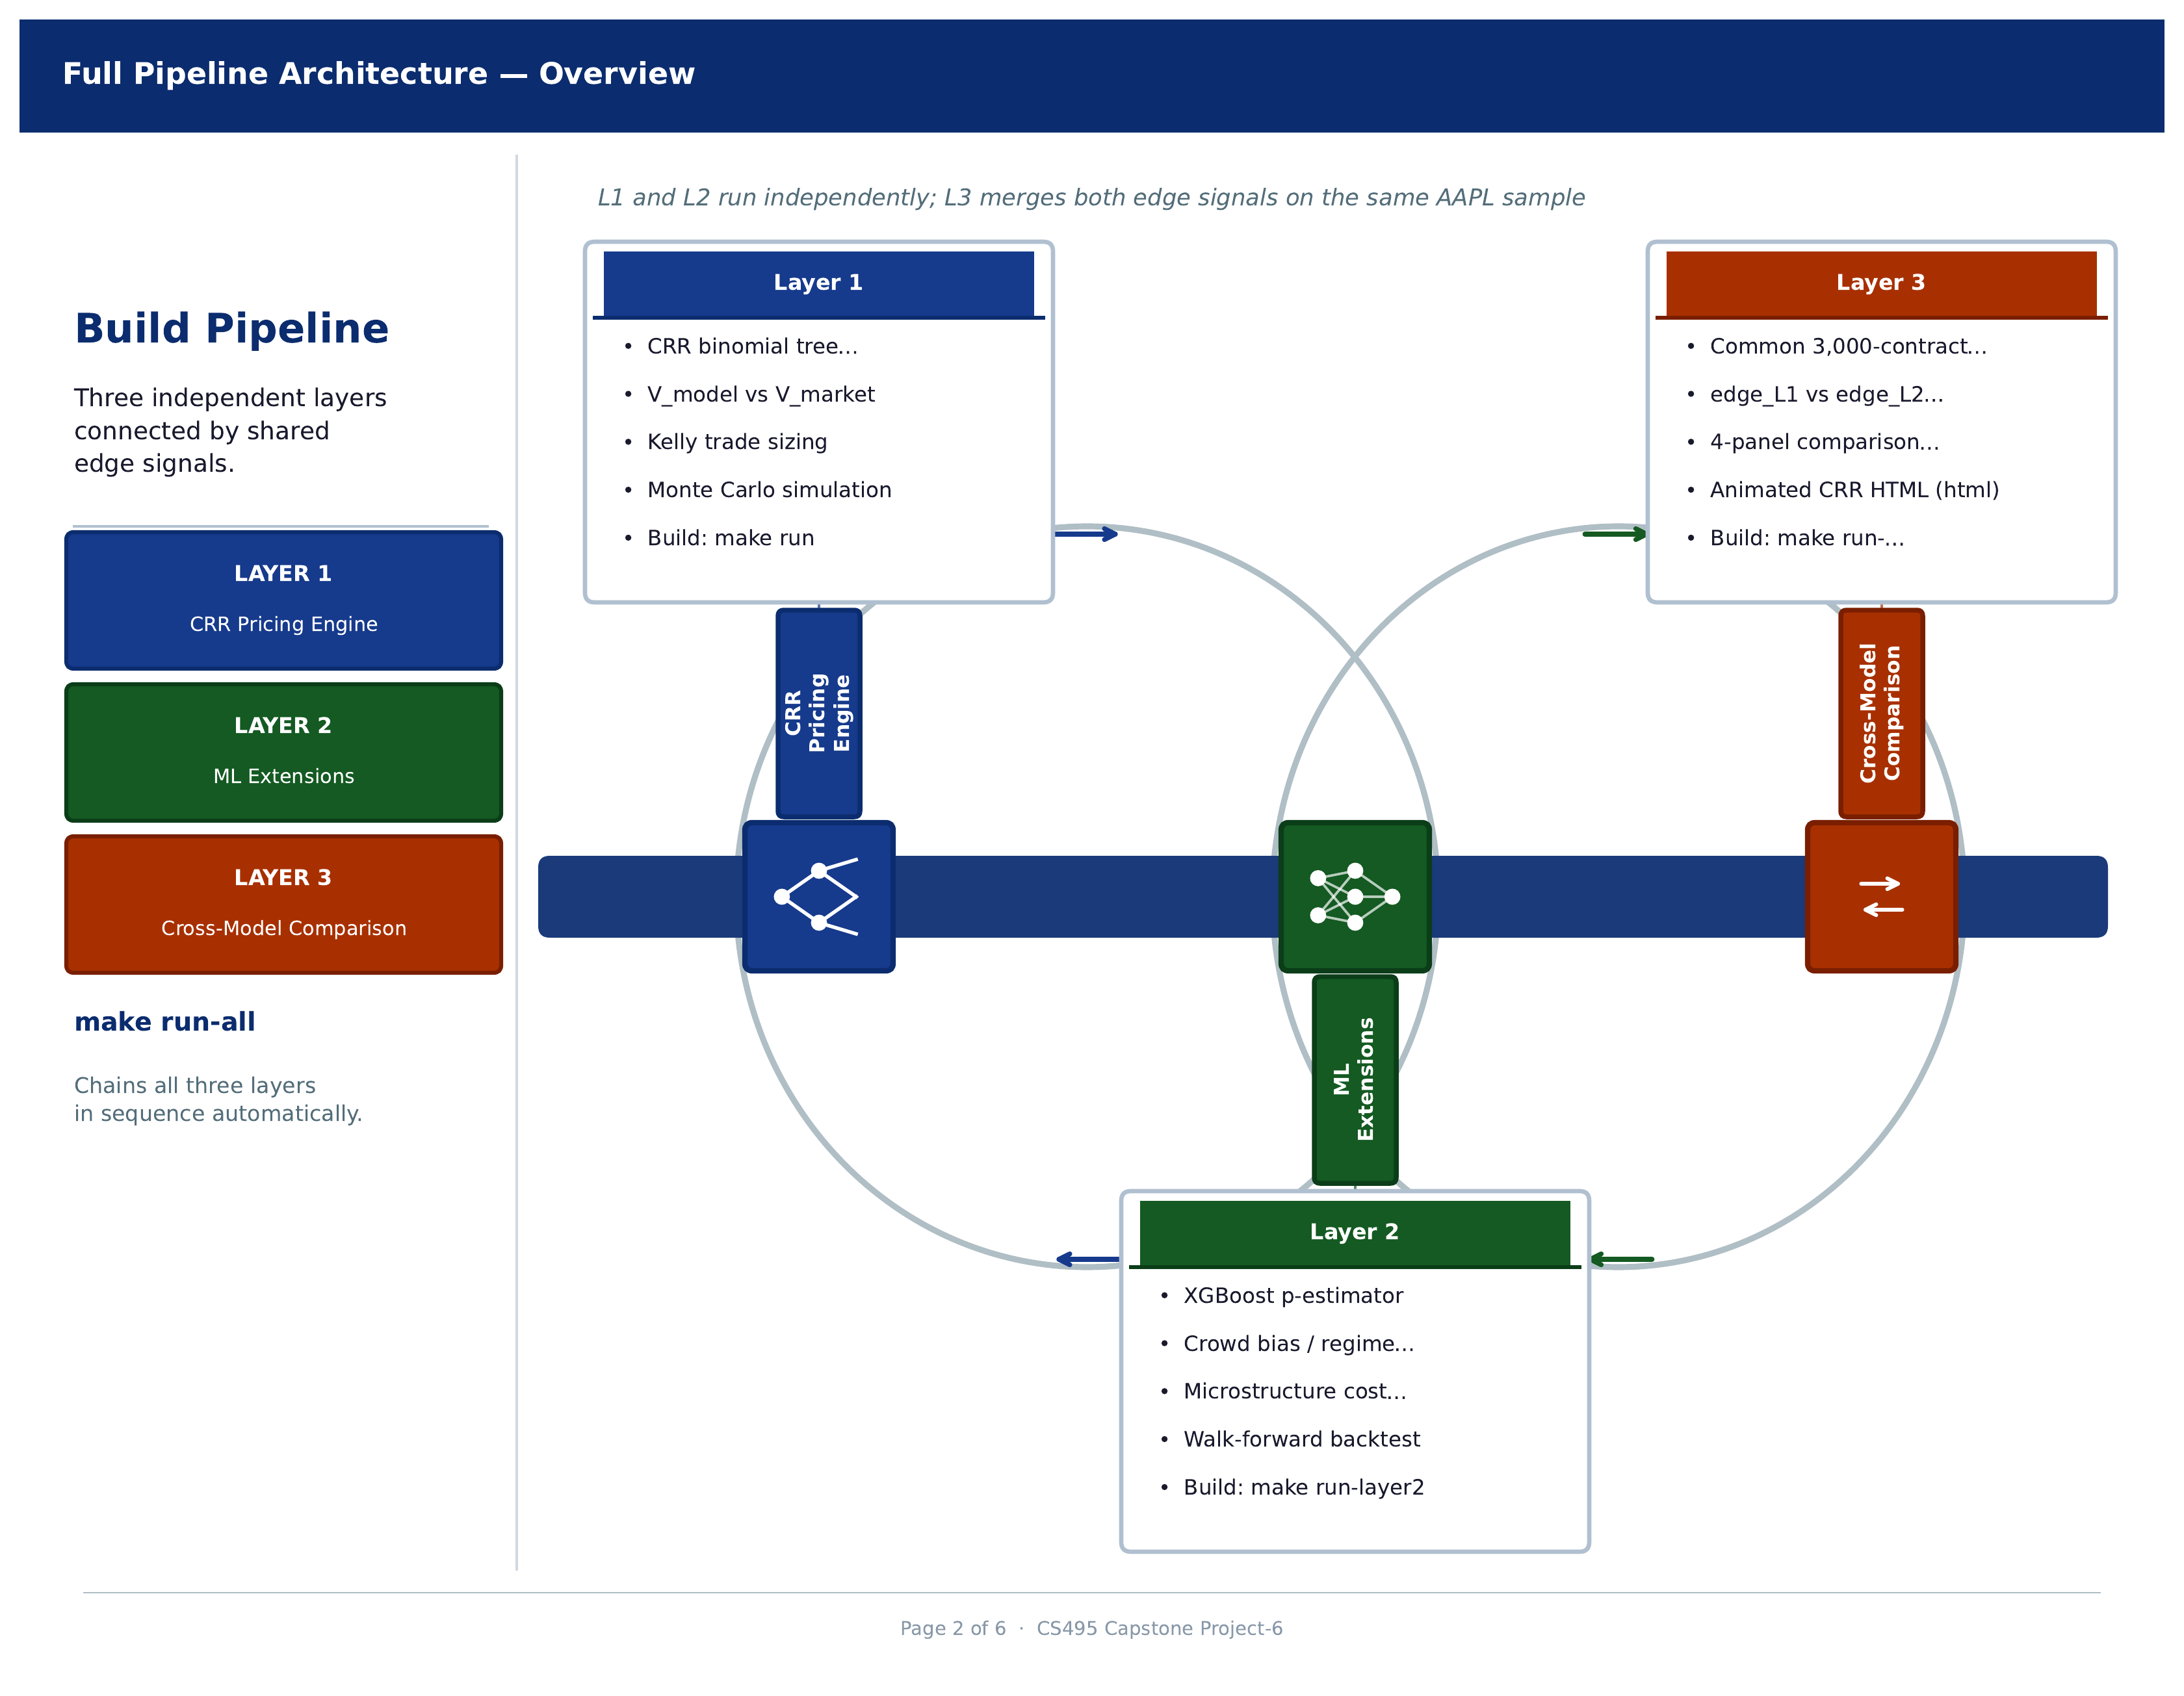
\includegraphics[width=0.72\linewidth,keepaspectratio]
    {PosterFigures/Flowchart-Slide2-Overview.png}
\end{center}

\vspace{0.4em}
\textbf{Techniques used}
\begin{itemize}[leftmargin=1.4em,itemsep=4pt,topsep=4pt]
  \item Vectorized recombining lattice in NumPy ($N{=}50$ to $100$ steps).
  \item Backward induction with American early-exercise check at each node.
  \item Greeks via centered finite differences.
  \item XGBoost trained on engineered features only ($\sigma$ input is
        RV30, never IV --- no leakage from L1).
  \item Platt scaling calibration; Brier-score validation.
  \item Walk-forward 60/20/20 split; zero look-ahead bias.
\end{itemize}
\end{posterblock}

\begin{posterblock}{Early Exercise Boundary}
The American-style optionality of the AMD put contracts is the
principal reason the CRR binomial lattice is required: Black--Scholes
omits early exercise. The boundary $S^{*}(t)$ is the critical stock
price at each day $t$ below which immediate exercise of the put
dominates holding to expiration. The figure overlays two cases drawn
from the lattice to isolate the regime in which the early-exercise
feature actually triggers.

\vspace{0.3em}
\begin{center}
  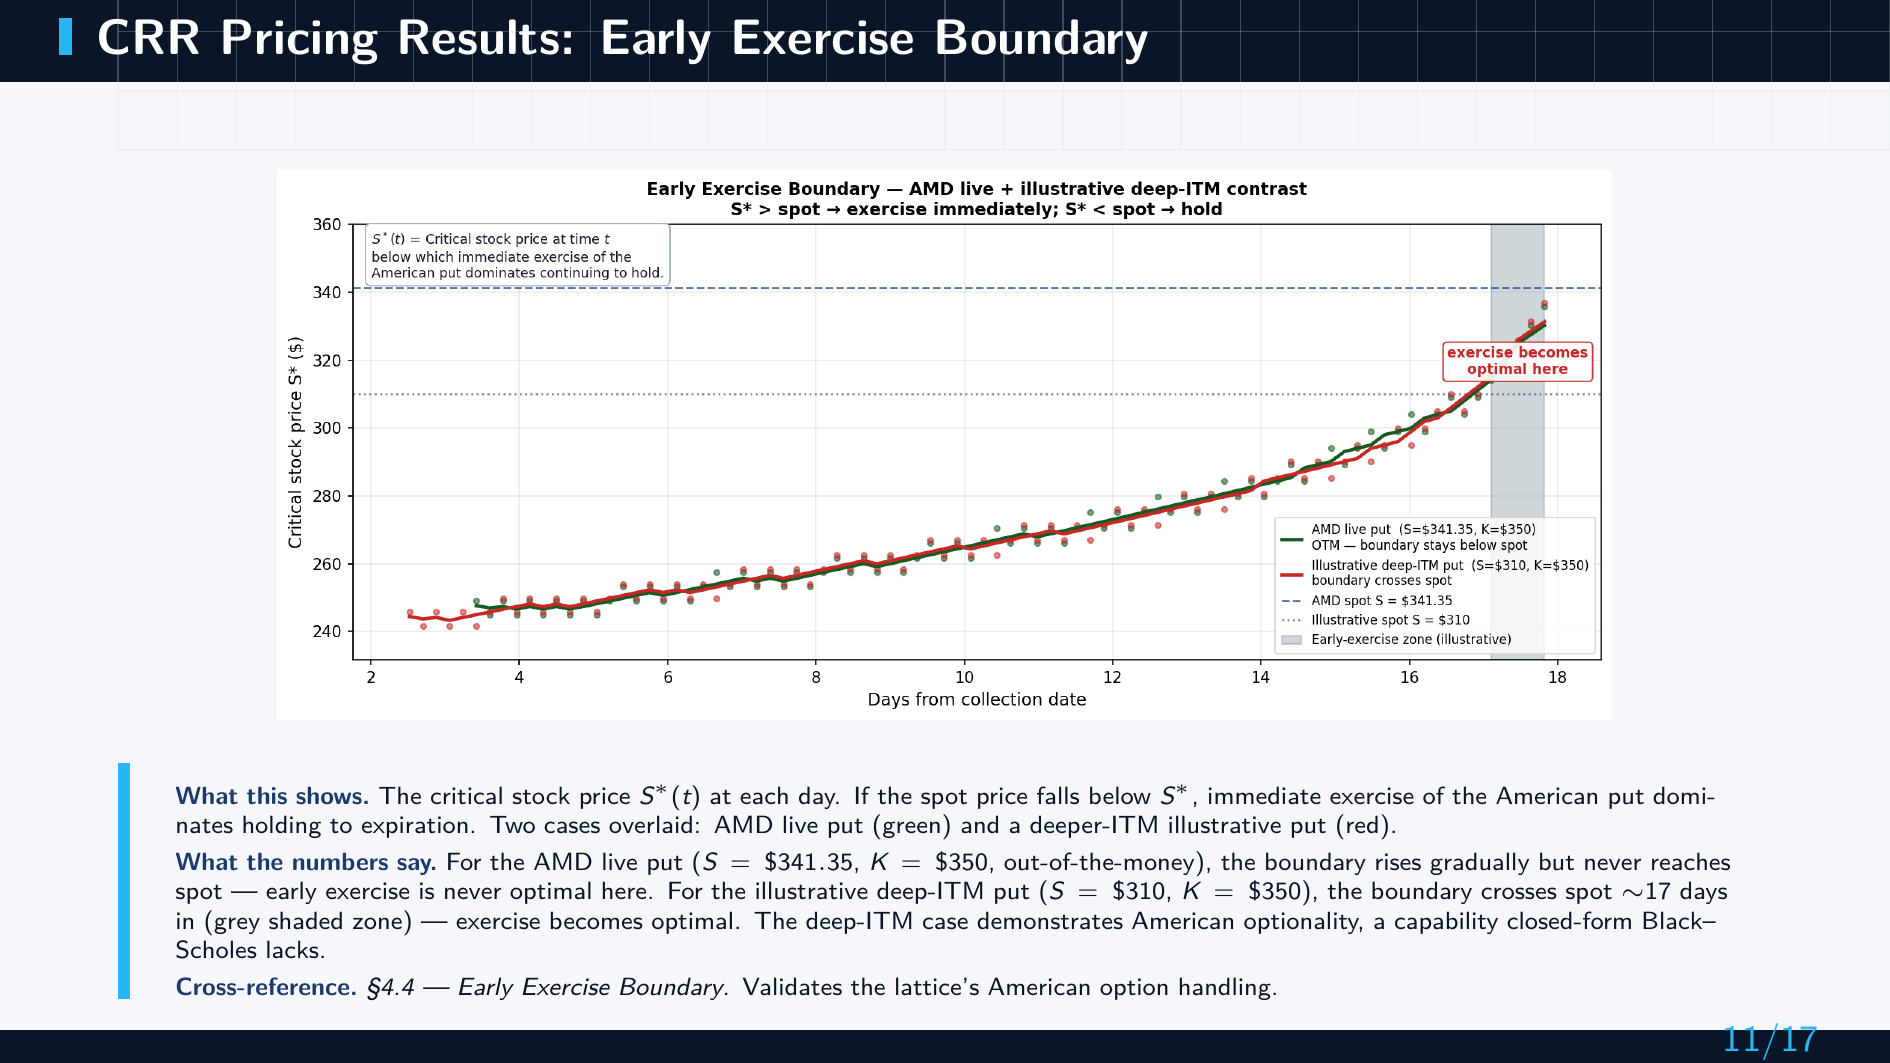
\includegraphics[width=0.78\linewidth,keepaspectratio]
    {PosterFigures/Slide11-EarlyExerciseBoundary.png}
\end{center}

\vspace{0.2em}
\textbf{AMD live put (green).} $S_{0}=\$341.35$ above $K=\$350$ ---
the boundary rises gradually but never reaches spot, so the
American premium exists in the model but never triggers as cash flow.

\vspace{0.2em}
\textbf{Deep-ITM put (red).} $S_{0}=\$310$ well below $K=\$350$ ---
the boundary crosses spot $\sim$17 days in (grey zone), at which
point early exercise becomes optimal. This isolates exactly the
contracts a European-only pricer would mishandle.
\end{posterblock}

\begin{posterblock}{Forward + Backward Pass}
\textit{Real AAPL put, 2020-03-16, herding regime
($S=\$241.47$, $K=\$240$, DTE $=18$d).}

\vspace{0.3em}
\noindent
\begin{minipage}[t]{0.49\linewidth}
\centering
\textbf{Forward Pass}\\[0.10em]
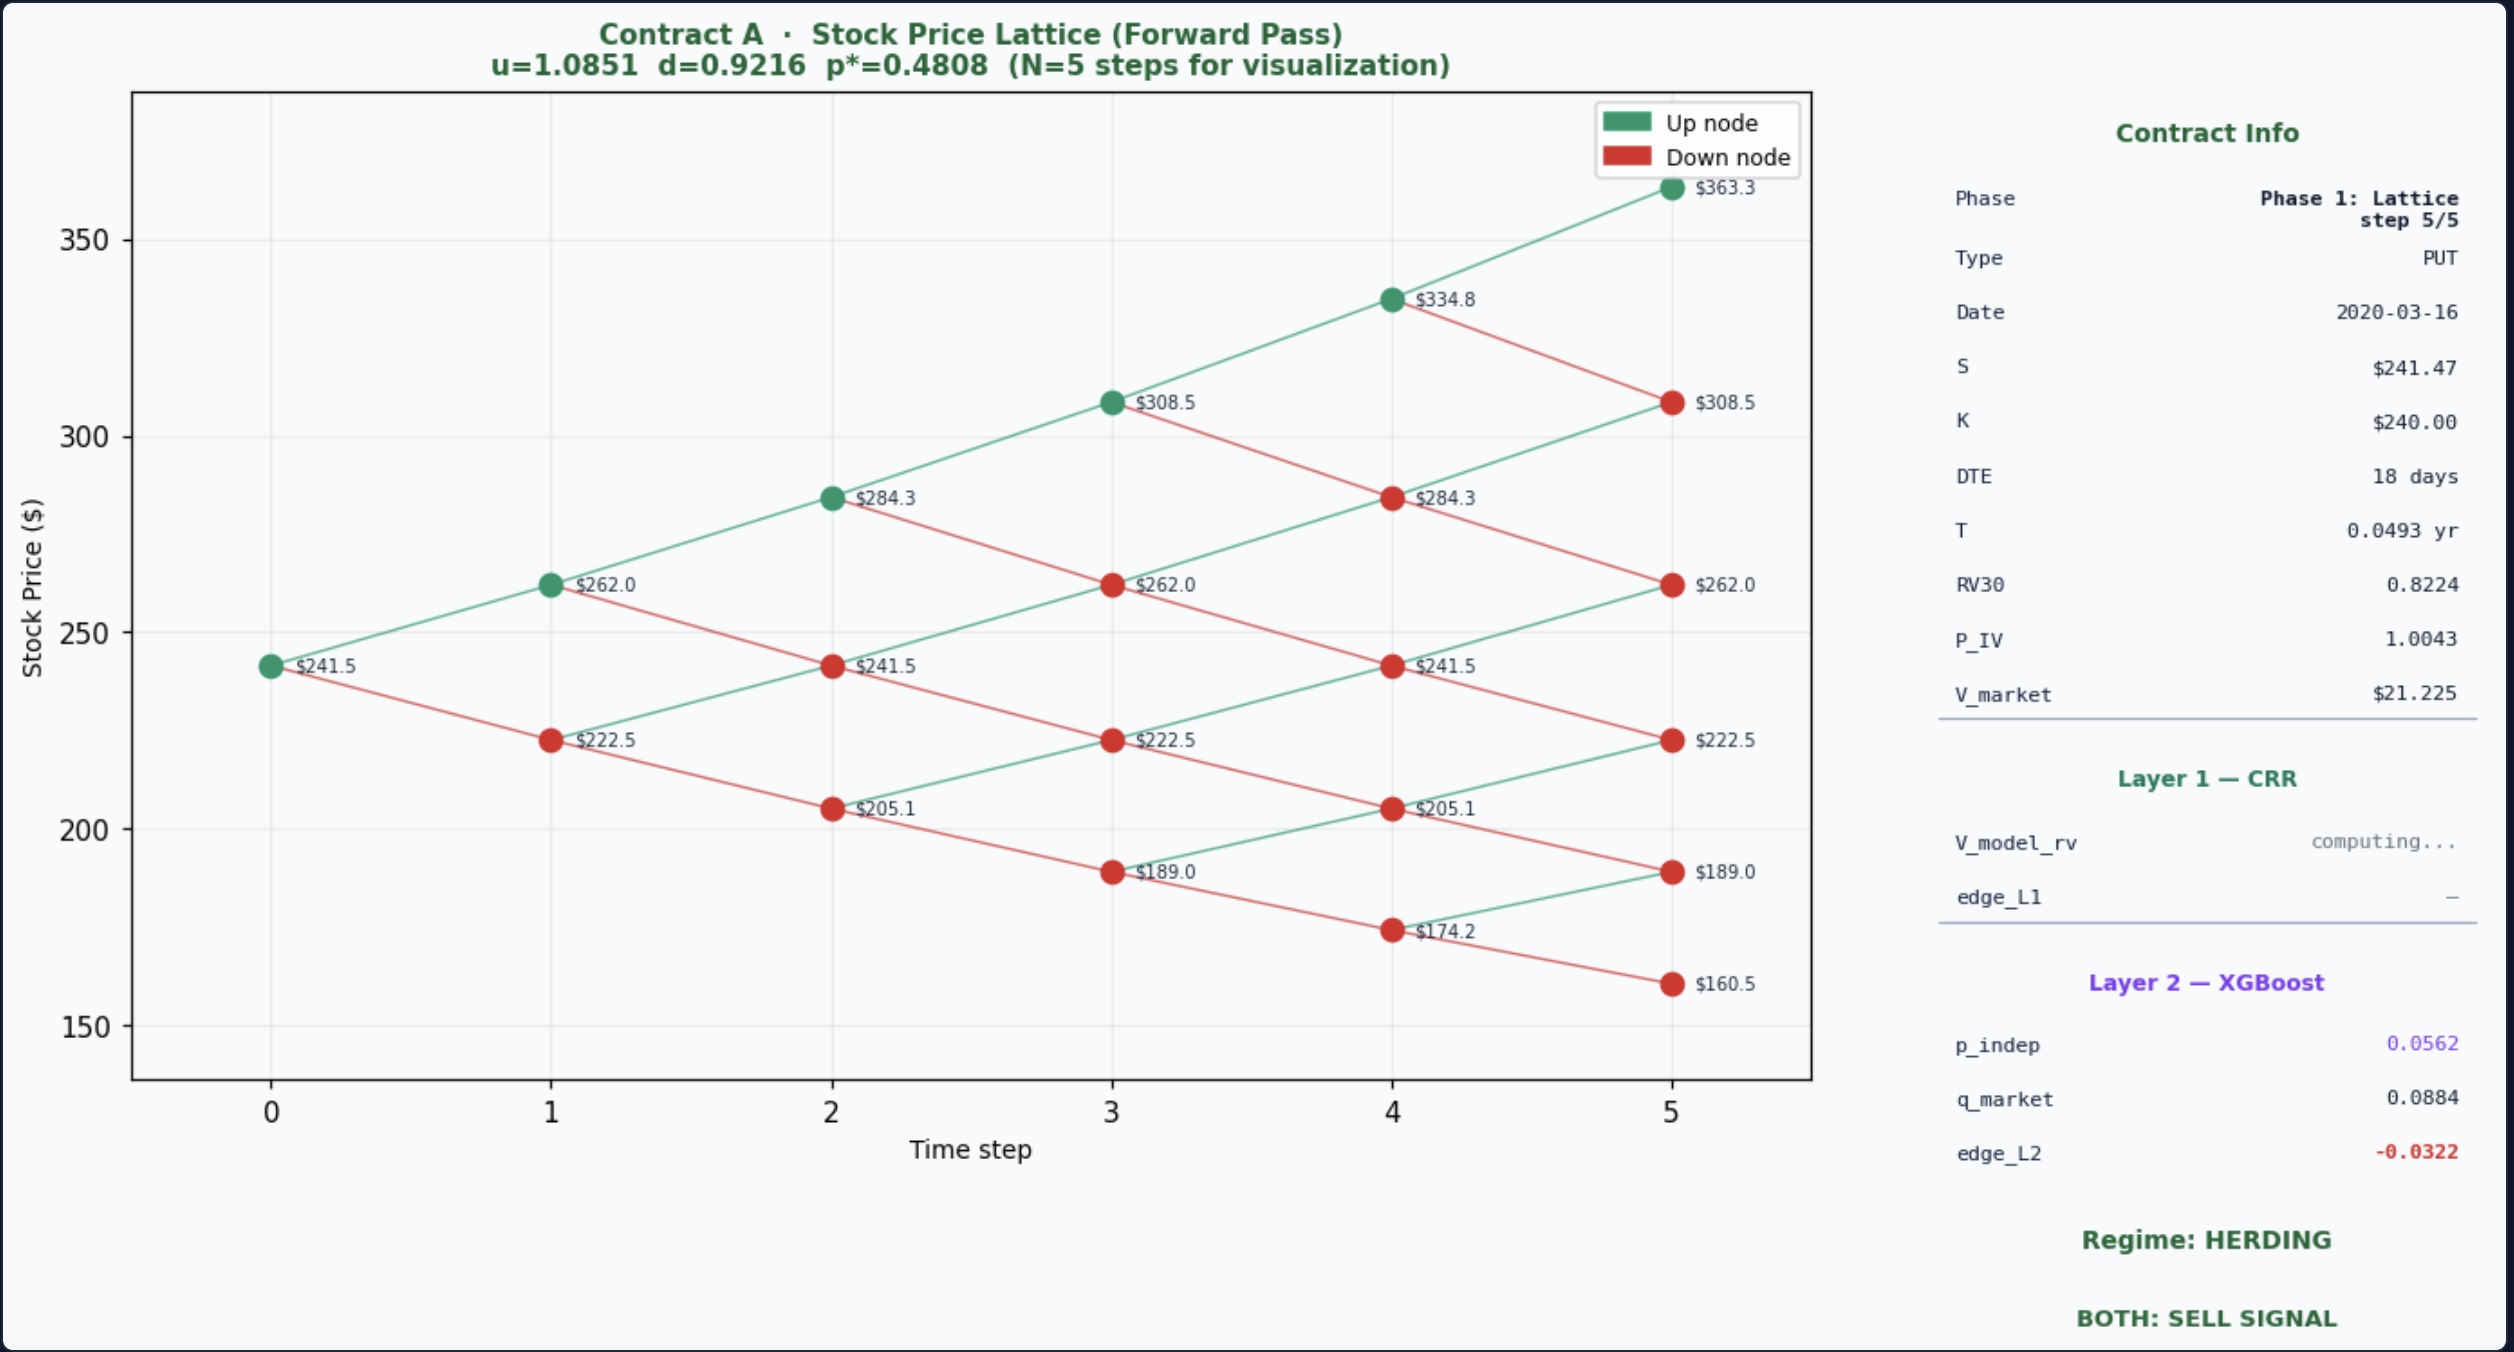
\includegraphics[width=\linewidth,keepaspectratio]
  {previews/Slide-Forward-Pass.png}
\end{minipage}\hfill
\begin{minipage}[t]{0.49\linewidth}
\centering
\textbf{Backward Induction}\\[0.10em]
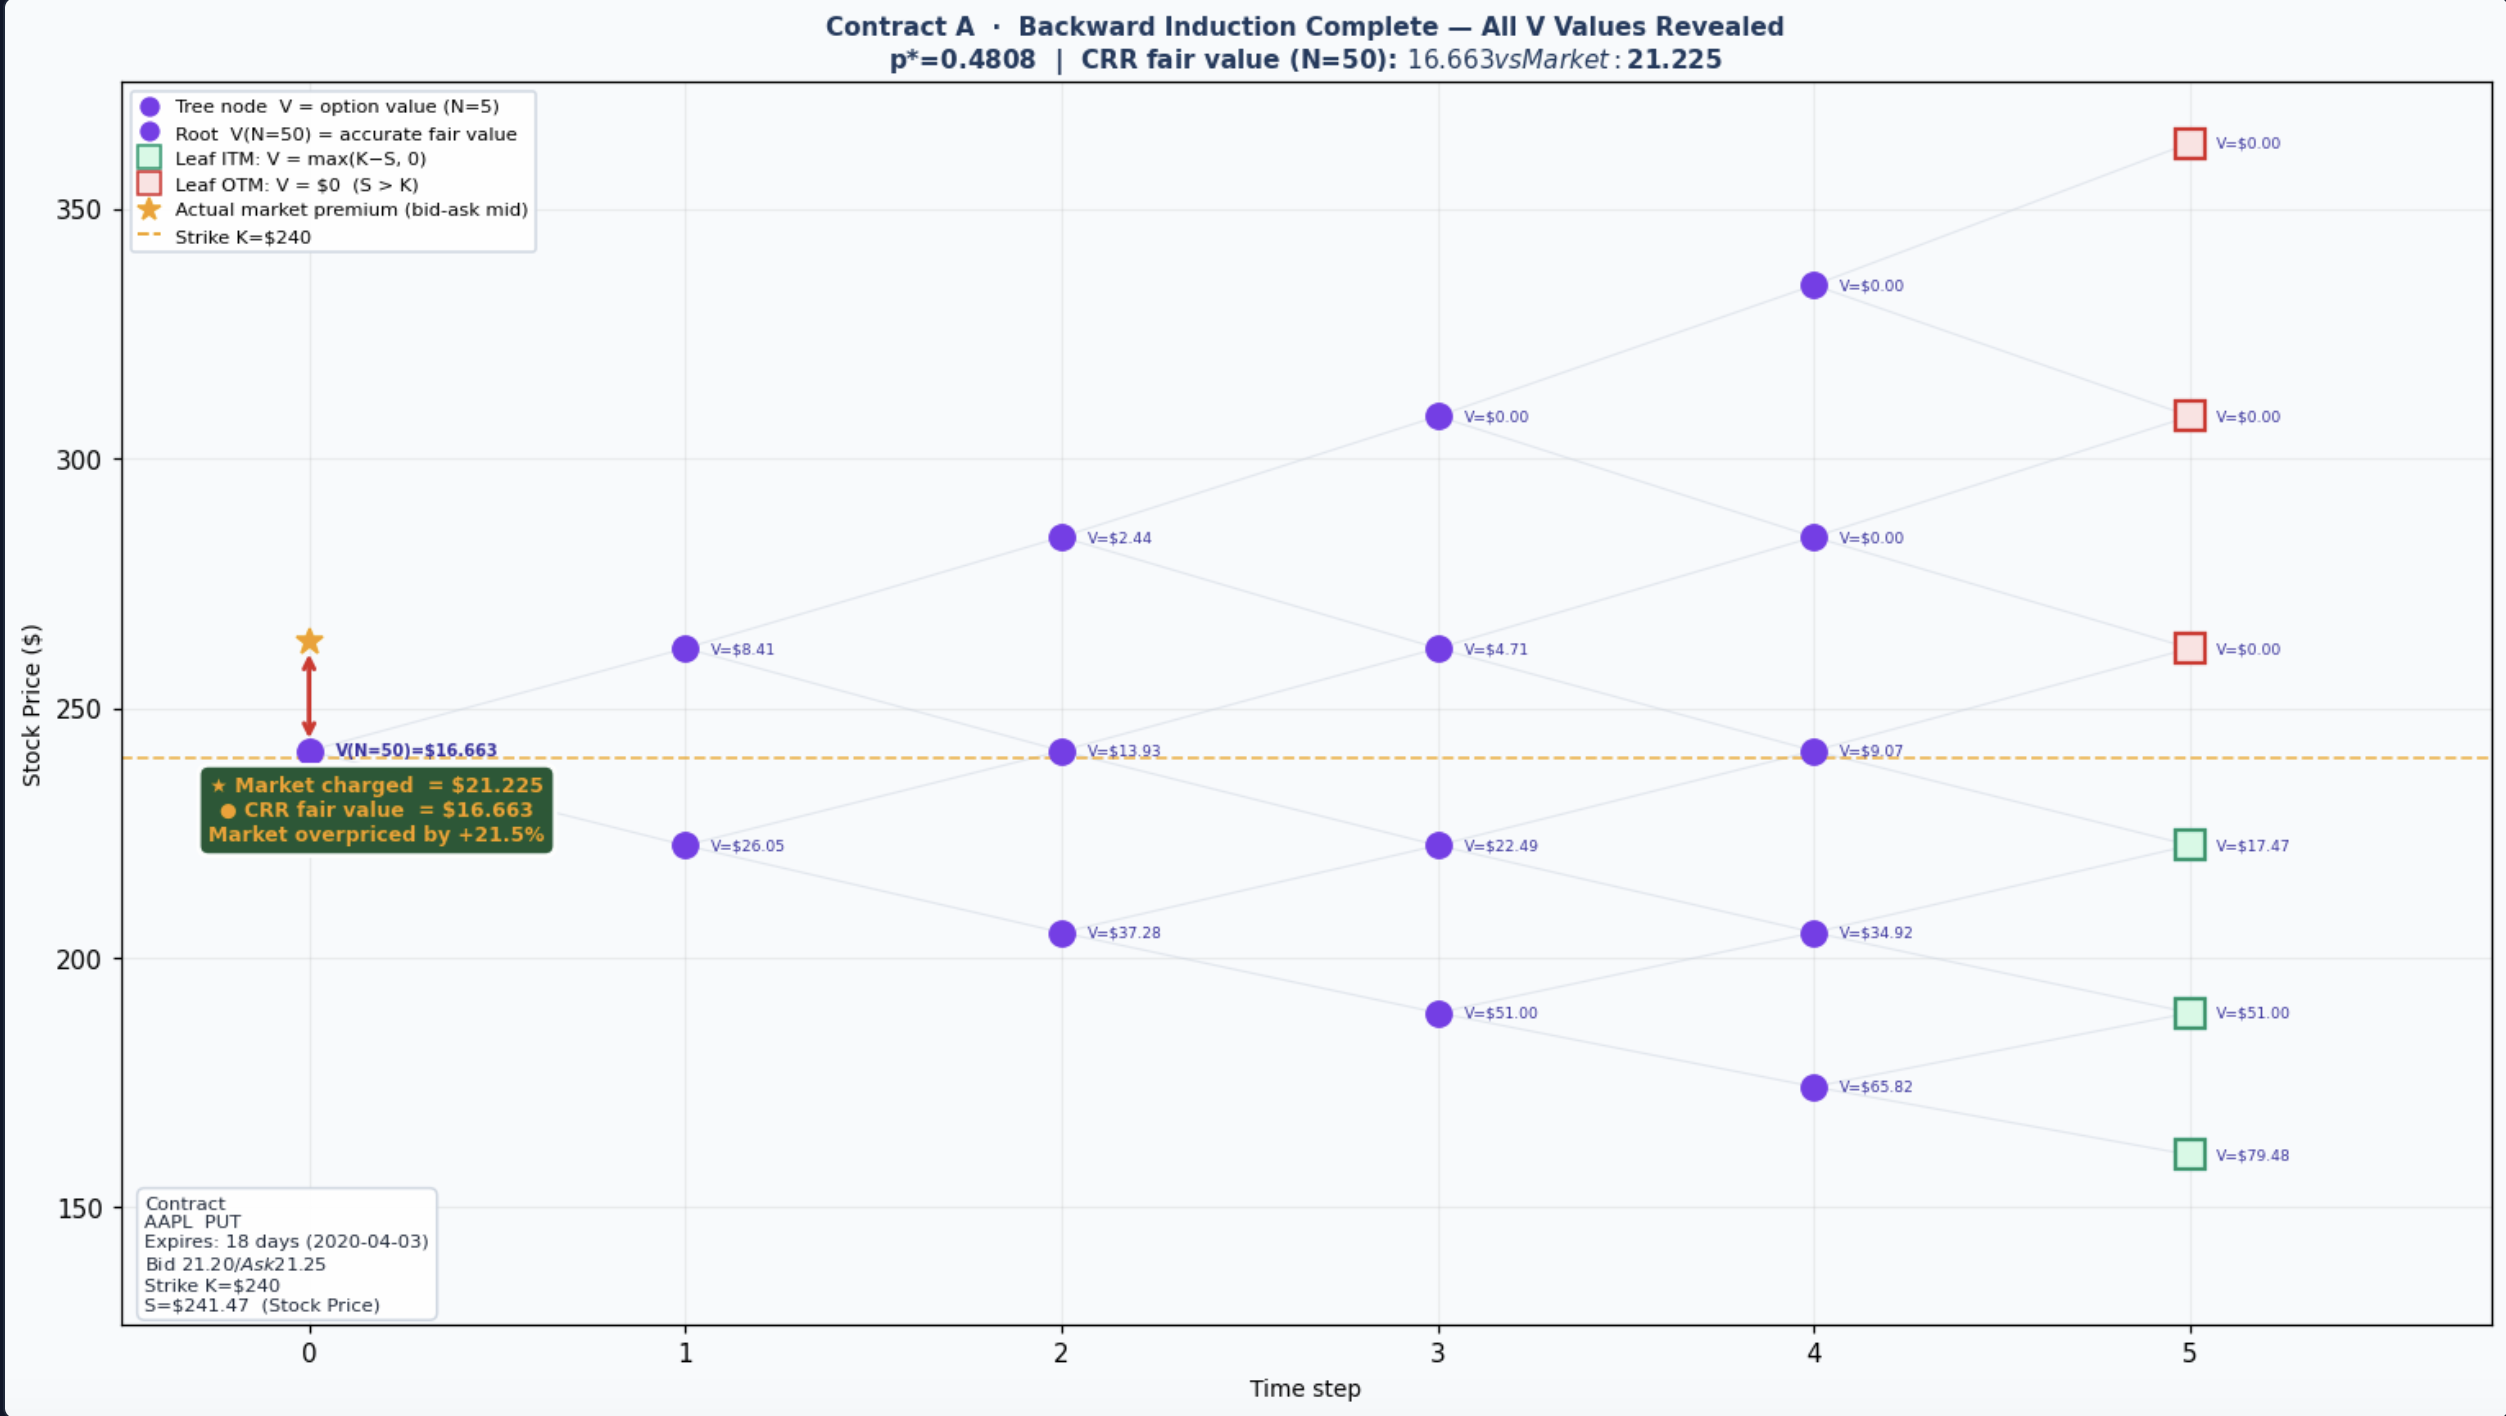
\includegraphics[width=\linewidth,keepaspectratio]
  {previews/Slide-Backward-Pass.png}
\end{minipage}
\end{posterblock}

\begin{posterblock}{Binomial Pricing Calculator}
An interactive Streamlit application packages the full Layer-1
pricing pipeline behind a ticker-agnostic front end: enter
$S$, $K$, DTE, $r$, $\sigma$, and the app renders the CRR tree
node-by-node, the model fair value, the edge against an entered
premium, the five Greeks, and the Kelly sizing recommendation.

\vspace{0.3em}
\begin{center}
  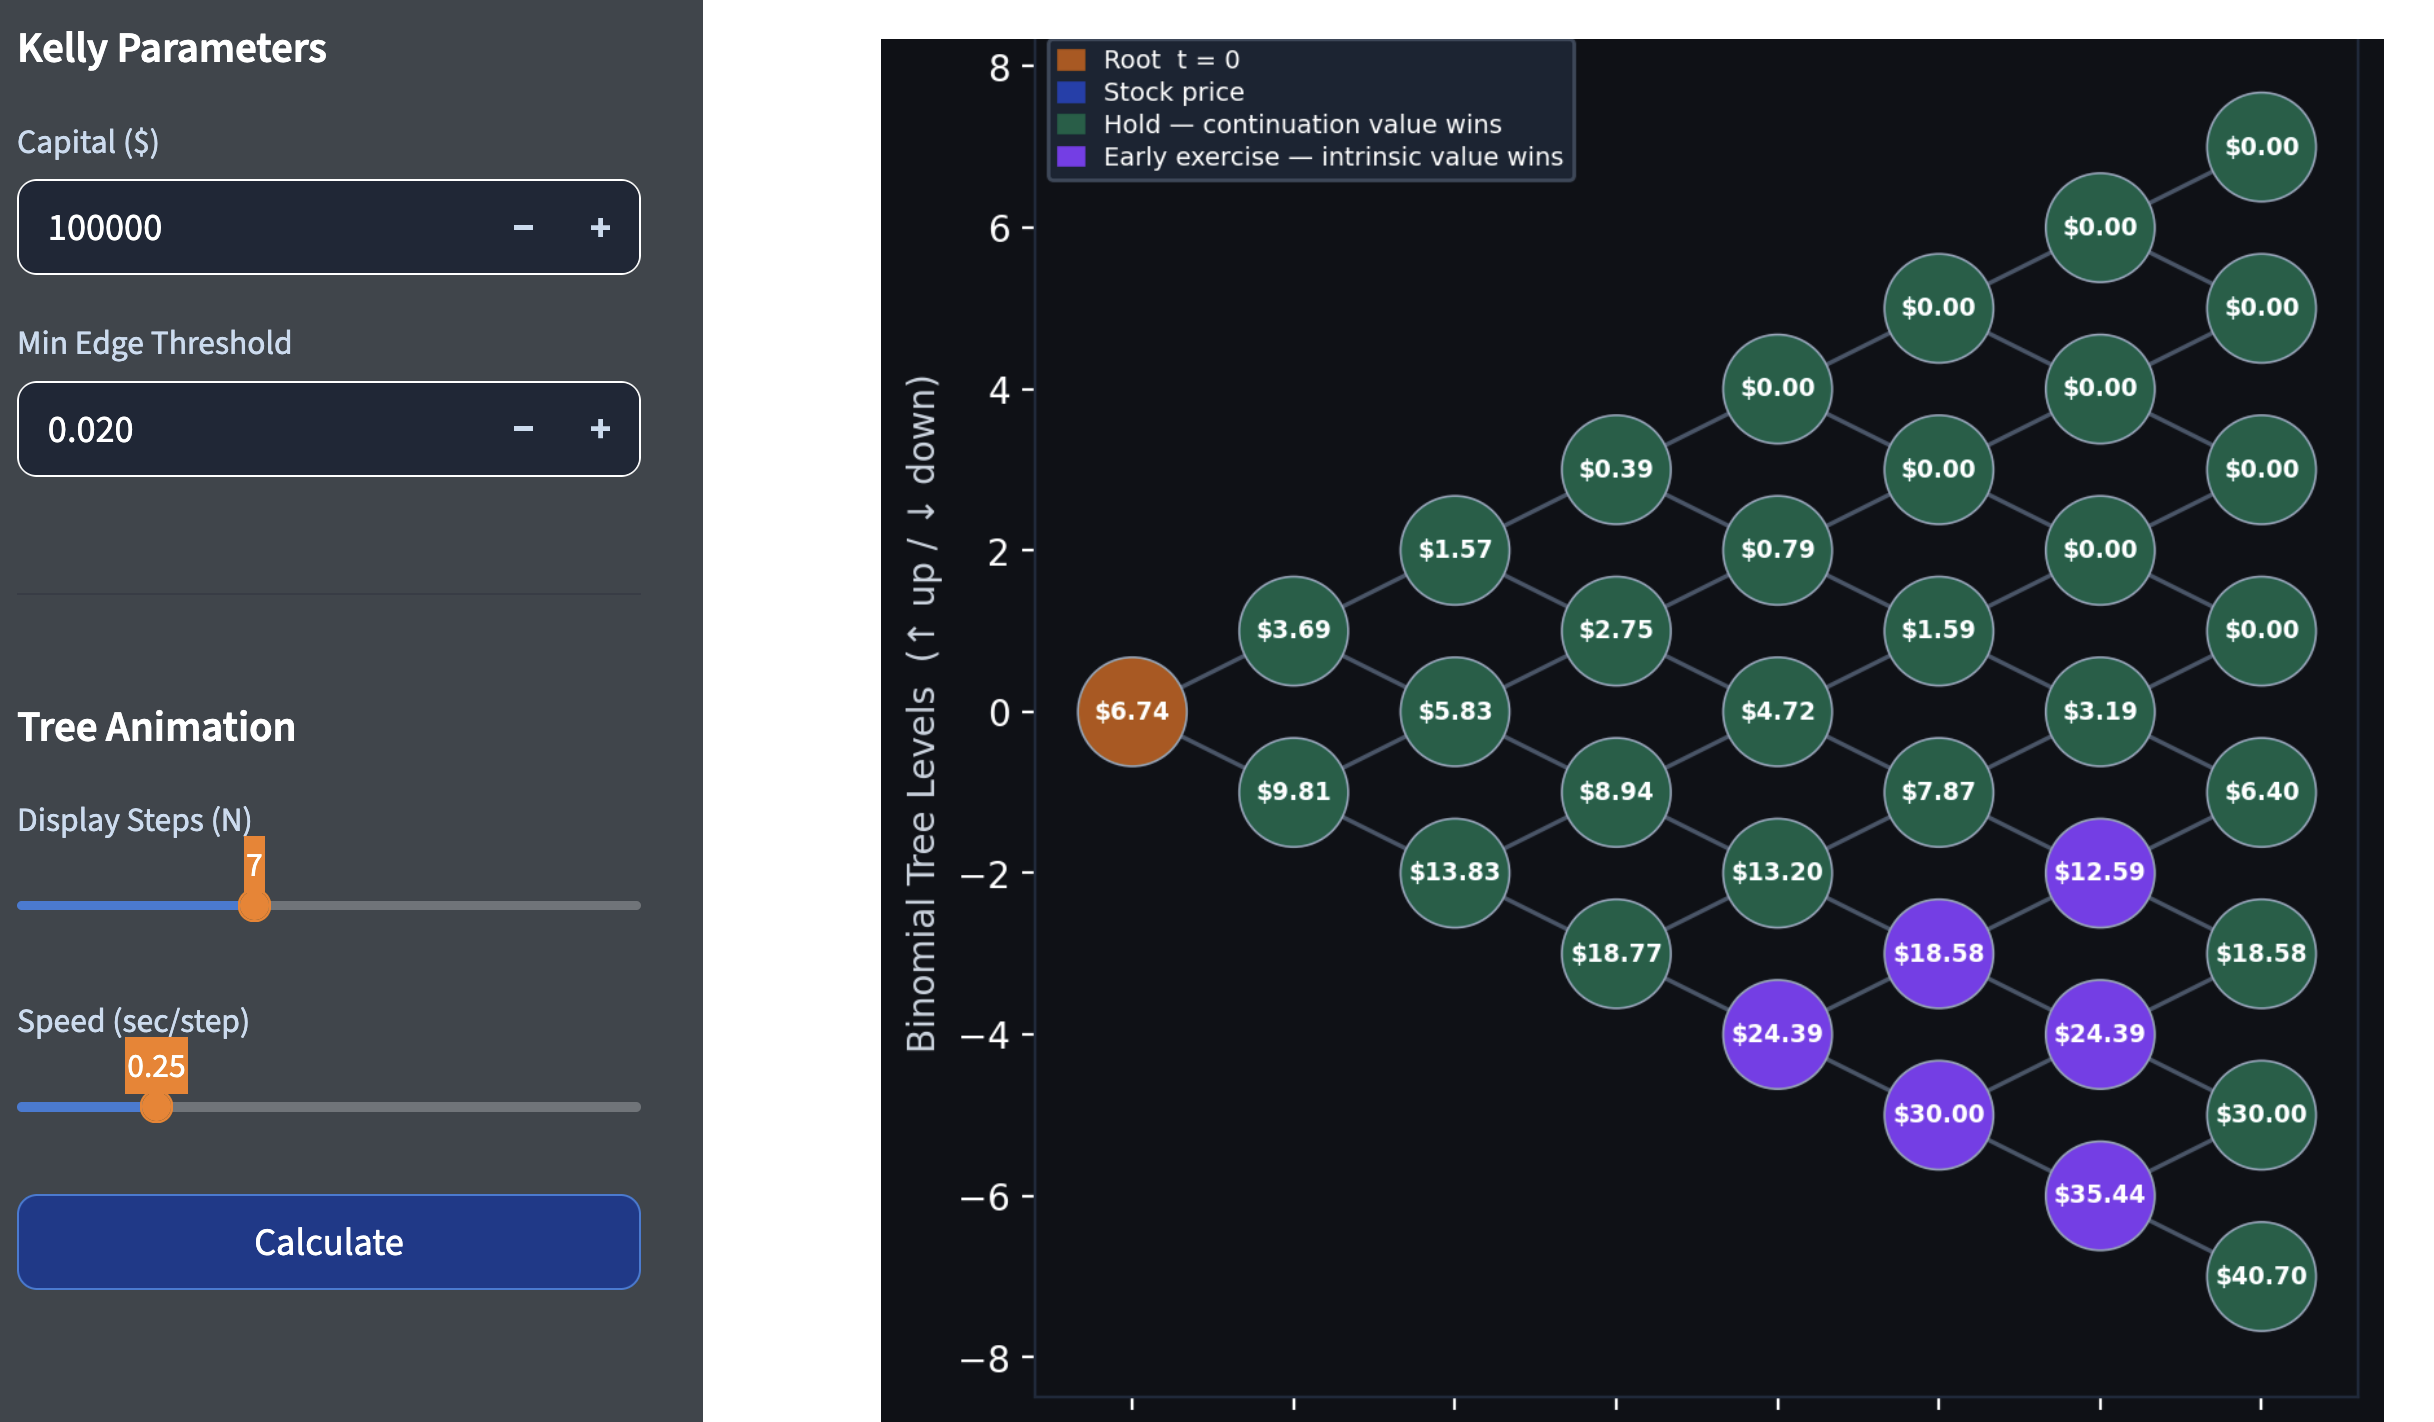
\includegraphics[width=0.78\linewidth,keepaspectratio]
    {PosterFigures/Binomial-Pricing-Calculator-Tree.png}
\end{center}

\vspace{0.2em}
\textbf{Tree visualization.} Each node shows
$S(i,j) = S_{0} \cdot u^{\,i-j} \cdot d^{\,j}$ from the forward
pass; the interactive animation then runs backward induction with
the American early-exercise check at every node, exposing the same
diagnostic the research pipeline uses.
\end{posterblock}

% ──────────────────────────────────────────────────────────────────────────────
\columnbreak
%  RIGHT COLUMN
% ──────────────────────────────────────────────────────────────────────────────

\begin{posterblock}{Results}
\textbf{Contract A} (real AAPL put, herding regime):
$S=\$241.47$, $K=\$240$, DTE $=18$d. Both independent models
arrive at the same trade decision:

\vspace{0.4em}
\begin{center}
  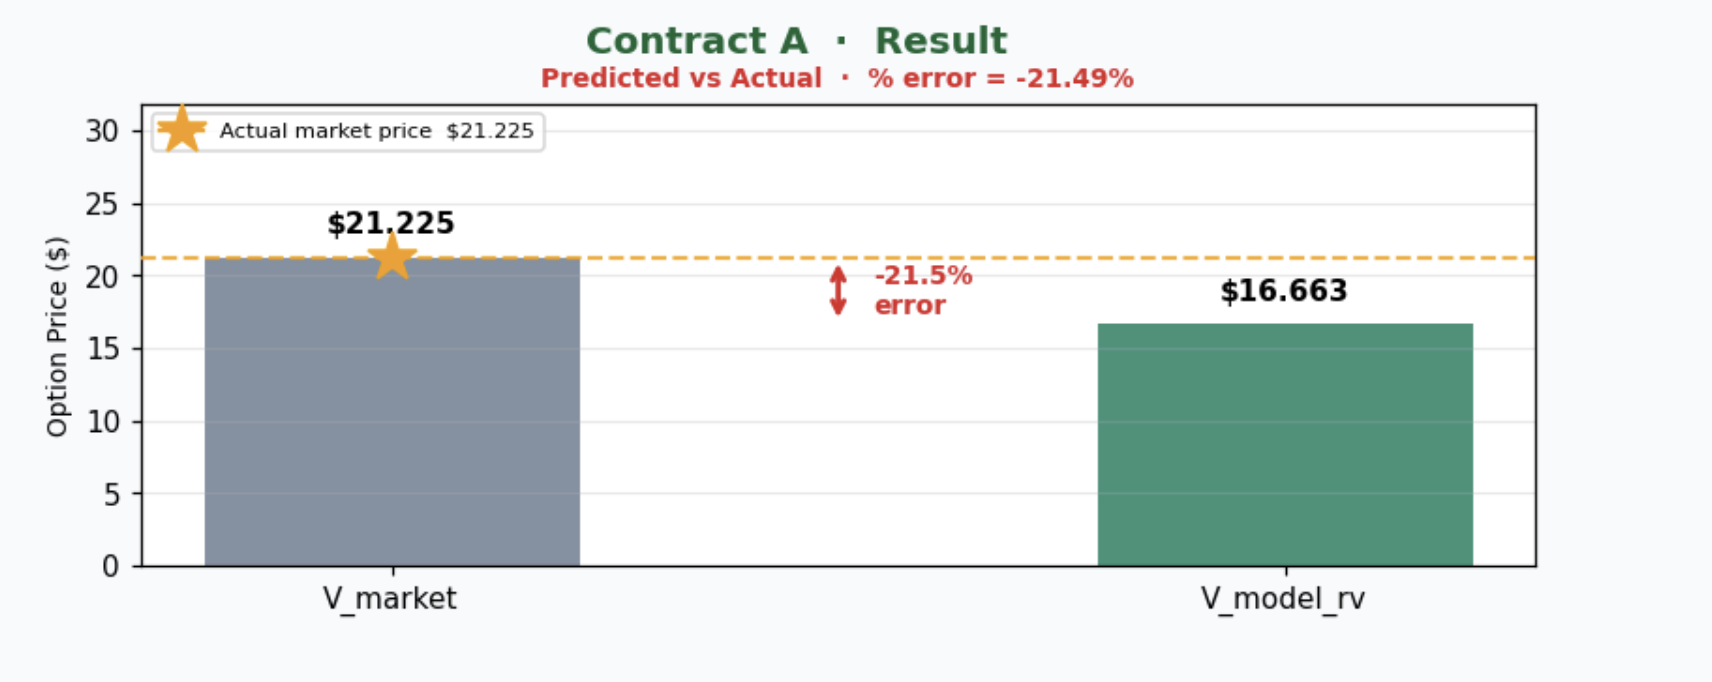
\includegraphics[width=0.92\linewidth,keepaspectratio]
    {PosterFigures/crr-binomial-contractA-herding-results.png}
\end{center}

\vspace{0.3em}
Layer 1 (CRR) edge $= -21.5\%$, Layer 2 (XGBoost) edge $= -3.2\%$:
\textbf{both layers say SELL} on this contract.

\vspace{0.6em}
\textbf{Performance summary} (101{,}535 AAPL contracts, walk-forward):

\vspace{0.3em}
\renewcommand{\arraystretch}{1.35}
\centering
\begin{tabular}{@{}lccc@{}}
\toprule
\textbf{Model} & \textbf{Brier} & \textbf{Hit rate} & \textbf{P\&L (\$)} \\
\midrule
Baseline (random)        & 0.250 & 50.0\%        & $0$         \\
Layer 1 CRR              & ---   & 63.0\%        & $+1.4$M     \\
Layer 2 XGBoost          & 0.211 & 66.5\%        & $+1.8$M     \\
\textbf{L1 $\cap$ L2 agree (Q3)} & --- & \textbf{76.5\%} & $+\mathbf{2.9}$M \\
\bottomrule
\end{tabular}
\RaggedRight

\vspace{0.6em}
\textbf{Cross-model agreement statistic:} Pearson correlation
coefficient $r = 0.413$ in herding regime ($n=217$,
$p = 2.4\times10^{-10}$); $r \approx 0$ in normal regime.
Max drawdown $<15\%$; \texttt{regime-conditioned} Kelly
(half-Normal, quarter-Herding) keeps risk bounded.
\end{posterblock}

\begin{posterblock}{Discussion \& Conclusions}
The central contribution is the \emph{cross-validation result}: two
\textbf{independent} models --- one mathematical (CRR no-arbitrage),
one empirical (XGBoost ML) --- detect the same mispricing direction
precisely in the regime behavioral finance theory predicts. Neither
layer is trained on the other; concurrent signals therefore come from
\emph{shared underlying reality}.

\vspace{0.5em}
\textbf{Answers to the Introduction's questions}
\begin{itemize}[leftmargin=1.4em,itemsep=4pt,topsep=4pt]
  \item \textbf{Yes --- CRR prices predict ITM/OTM.} Layer-1 alone
        achieves a $63\%$ per-trade hit rate on $101{,}535$ AAPL
        contracts; Layer-2 (XGBoost) drives Brier score to $0.211$,
        below the $0.25$ naïve baseline.
  \item \textbf{Yes --- cross-validation detects exploitable edge.}
        Pooled $r=0.032$ collapses to $r=\mathbf{0.413}$
        ($p=2.4\times10^{-10}$, $n=217$) once the herding regime is
        isolated --- a Simpson's paradox in which both-SELL contracts
        (Q3) realize a $76.5\%$ ITM rate vs.\ the $\sim 63\%$ baseline.
  \item \textbf{Yes --- regime-conditioned Kelly converts edge into
        positive expected value.} Walk-forward backtest produces
        $\mathbf{\$2.94}$M cumulative P\&L on a \$100k base across
        $3{,}760$ executed trades ($63.1\%$ hit rate, max drawdown
        $<15\%$, circuit breaker never fired).
  \item The framework's most valuable output is the \emph{no-trade}
        signal --- when CRR and XGBoost disagree, no position is taken.
\end{itemize}

\vspace{0.3em}
\textbf{Limitations.} AAPL 2016--2020 is a single equity in a single
market cycle; CRR uses a flat IV per contract (no smile / skew);
backtest assumes mid-price fills with no transaction friction; regime
detection is backward-looking via IV/RV$_{30}$.

\vspace{0.3em}
\textbf{Future work.} Expand to SPY / QQQ / NDX options; integrate
LSTM volatility forecaster; live paper-trading via IBKR / Alpaca;
multi-leg spreads (vertical, calendar, iron condor) with joint Kelly
sizing.
\end{posterblock}

\begin{posterblock}{References}
\normalsize
\begin{enumerate}[leftmargin=1.6em,itemsep=4pt,topsep=4pt]
  \item Black, F. \& Scholes, M. (1973). The Pricing of Options and
        Corporate Liabilities. \emph{Journal of Political Economy} 81(3),
        637--654.
  \item \textbf{Cox, J., Ross, S., \& Rubinstein, M.} (1979). Option
        Pricing: A Simplified Approach. \emph{Journal of Financial
        Economics} 7(3), 229--263.
  \item \textbf{Fama, E.\,F.} (1970). Efficient Capital Markets:
        A Review of Theory and Empirical Work. \emph{Journal of
        Finance} 25(2), 383--417.
  \item \textbf{Wrigglesworth, A.} (2020). The CRR Binomial Option
        Pricing Model: An Analysis of Accuracy, Convergence and
        Stability Using Python. University of Pretoria, 30 April 2020.
  \item Carr, P. \& Wu, L. (2009). Variance Risk Premiums.
        \emph{Review of Financial Studies} 22(3), 1311--1341.
  \item Kelly, J.\,L. (1956). A New Interpretation of Information Rate.
        \emph{Bell System Technical Journal} 35(4), 917--926.
  \item MacLean, L., Thorp, E.\,O. \& Ziemba, W. (2010). Good and Bad
        Properties of the Kelly Criterion. \emph{Quantitative Finance}
        10(1), 7--14.
\end{enumerate}
\end{posterblock}

\begin{posterblock}{Acknowledgments \& Contact}
The author thanks \textbf{Dr.~Pedro Albuquerque} for his guidance
throughout CS\,495, and the Bellevue College Computer Science program
for supporting this capstone project.

\vspace{0.4em}
\textbf{Contact:} \texttt{dewayne.dantzler@bellevuecollege.edu}\\
\textbf{Code / Repository:}
\texttt{github.com/dantzlerdc/CS495-Deep-Scholar}

\vspace{0.3em}
\begin{center}
\fbox{\qrcode[height=3cm]{https://github.com/dantzlerdc/CS495-Deep-Scholar}}
\\[0.2em]
\small\textit{Scan to open the full repository}
\end{center}
\end{posterblock}

\end{multicols}

% ══════════════════════════════════════════════════════════════════════════════
%  FOOTER BAND  (overlay anchored to the page so it always sits at the bottom)
% ══════════════════════════════════════════════════════════════════════════════
\begin{tikzpicture}[remember picture, overlay]
  \fill[BCBlue] ([yshift=0.4cm]current page.south west)
                rectangle ([yshift=1.8cm]current page.south east);
  \fill[BCRed]  ([yshift=1.8cm]current page.south west)
                rectangle ([yshift=2.0cm]current page.south east);
  \node[anchor=west, white] at ([xshift=1cm, yshift=1.1cm]current page.south west)
    {\bfseries\Large CS\,495 -- Data Science Project Practicum};
  \node[anchor=east, white] at ([xshift=-1cm, yshift=1.1cm]current page.south east)
    {\Large Bellevue College \;\textbullet\; Spring 2026};
\end{tikzpicture}%

\end{document}
